\documentclass{article}
\usepackage[utf8]{inputenc}
\usepackage{latexsym}
\usepackage{url}
\usepackage{hyperref}
\usepackage{graphicx}
\usepackage[table]{xcolor}
%\usepackage{enumitem,amssymb}
%\usepackage{txfonts}

\usepackage[utf8]{inputenc} % Required for inputting international characters
\usepackage[T1]{fontenc} % Output font encoding for international characters

\usepackage{mathpazo} % Palatino font

\begin{document}

\begin{titlepage} 
	\newcommand{\HRule}{\rule{\linewidth}{0,6mm}}
	
	\center
	
	\textsc{\huge Proiectarea Algoritmilor}\\[5cm] 

	\HRule\\[0.8cm]
	
	{\Huge\bfseries Selectarea aspersoarelor}\\[0.6cm] % Title of your document
	
	\HRule\\[1.9cm]
   
	\vspace{20mm}
	\begin{minipage}{1\textwidth}
		\begin{flushleft}
	        \centering
			\huge
			\textbf{Studenta}: \textsc{Bădiță Georgiana - Elena}\\
			 \textbf{Grupa} : CR1.1A\\
			 \textbf{An} : I\\
			 \textbf{Specializarea} : Calculatoare română\\
			
			
		\end{flushleft}
	\end{minipage}
\end{titlepage}


%\maketitle
\newpage


\section{Enunțul problemei}
\textbf {Selectarea aspersoarelor}. Se consideră \textsl {n} aspersoare instalate să ude o
bandă  orizontală de iarbă ce are \textsl{L} metri lungime și \textsl{l} metri lățime. Fiecare aspersor este centrat vertical pe banda de iarbă respectivă. Pentru fiecare aspersor se cunosc: i) poziția sa ca distanță față de capătul din stânga  al liniei care străbate  pe orizontală mijlocul fâșiei de iarbă  și respectiv ii)raza sa de operare. Să se determine numărul minim de apsersoare care trebuie pornite pentru a putea uda întreaga bandă de iarbă. Implementați
doi algoritmi diferiți.

\vspace{5mm}

\section{Algoritmii propuși}

\\ 
\textbf{Fișierul \textit{functions.c}}\\
\textbf{Algoritm I \\
\textsl{Metoda I}}

\vspace{6mm}
\caption{Pseudo-codul funcției \textbf{minAspensNumber}, cea care determină care este numărul minim de aspersoare ce trebuie pornite pentru a putea uda banda de iarbă.} \vspace{6mm}
\\
\begin{algorithm}
\begin{algorithmic}[1]
MIN-ASPENS-NUMBER() \\
1.\indent   \>$init minAspens = 1$ \\
2.\indent   \>$init startIndex = 0$ \\
3.\indent   \>$init index = 1$\\
4. \indent            \> $\textbf{while} $index < aspenTotal$ and aspenPositionArray_{index}.start = 0 $ \textbf{do} \\
5. \indent            \> \hspace{8mm}   \>  $\textbf{if} $ aspenPosition_{index}.start = 0$  $\textbf{and} $   $aspenPositionArray_{startIndex}.end $ \\
\indent   \> \hspace{16mm}\> < $ aspenPositionArray_{index}.end$ \\
6. \indent            \>\hspace{16mm} $startIndex = index$ \\
7.\indent             \> \hspace{8mm}    \> $\textbf{end if }$\\
8. \indent            \>\hspace{4mm}  $index = index + 1$ \\
9.\indent             \> $\textbf{end while}$\\
10. \indent            \>$currentIndex = startIndex$ \\
11.\indent \>$\textbf{while} aspenPositionArray_{currentIndex}.end$$<$$length$$ \textbf{and}$ $currentIndex$$<$$aspenTotal$$\textbf{do}$\\
12.\indent                \>\hspace{17mm}$nextIndex = currentIndex$\\
13.\indent                 \>\hspace{17mm}$index = currentIndex + 1 $\\
14.\indent            \> \hspace{8mm}$\textbf{while}$  $ aspenPositionArray_{index}.start $ $<$ $ aspenPositionArray_{currentIndex}.end$\\  
\indent       \> \hspace{17mm} \> $\textbf{and} $ $index$ < $ aspenTotal $ \textbf{do}$ \\
15.\indent            \>\hspace{18mm} $\textbf{if} $ $  aspenPositionArray_{index}.start $ $ <$   $ aspenPositionArray_{currentIndex}.end $ 
\indent               \>\hspace{25mm}$\textbf{and}$ $ aspenPositionArray_{nextIndex}.end$$ <$ aspenPositionArray_{index}.end $ 
16.\indent                \>\hspace{26mm} $nextIndex = index$\\
17.\indent      \>\hspace{18mm} $\textbf{end if}$\\
18.\indent \>\hspace{18mm}$index = index + 1$ \\
19.\indent    \>\hspace{8mm}$\textbf{end while}$\\
20.\indent                \>\hspace{8mm} $\textbf{if} $ $currentIndex \neq nextIndex$ \\
21.\indent                \>\hspace{18mm} $currentIndex = nextIndex$\\
22.\indent                 \>\hspace{18mm} $minAspens = minAspens + 1$\\
23.\indent  \> \hspace{8mm} $\textbf{end if} $\\
24.\indent                 \>\hspace{8mm} $\textbf{then}\\
25.\indent                 \>\hspace{12mm} $\textbf{break}\\
26.\indent            \> $\textbf{end while}$\\
27.\indent            \> $\textbf{if} aspenPositionArray_{currentIndex}.end $ $ <$  $ length$ \\
28.\indent           \>\hspace{8mm} $minAspens = - 1 $ \\
29.\indent               \>$\textbf{end if}$\\
30.\indent          \>$\textbf{return} minAspens$\\

\end{algorithmic}
\end{algoritm}
\vspace{4mm}
Inainte de a fi apelată această funcție în \textbf{main.c}, a mai fost apelată și funcția \textbf{arrayAspenToArrayAspenPosition}, o funcție care convertește fiecare element ce se regăsește în vectorul numit \textit{aspenArray} în tipul \textit{aspenPosition} și memorează în vectorul numit \textit{aspenPositionArray}.Acest vector \textbf{aspenPositionArray}, care este unul de tipul \textit{struct aspenPosition}, memorează pentru fiecare aspersor începutul și sfârșitul de unde până unde  udă cu exactitate aspersorul ( acest lucru este exemplificat în \textit{Figura 2} de mai jos). De asemenea, fiecare aspersor a fost sortat prin metoda \textit{Bubble-sort}(o metodă de sortare ce are ca și timp de complexitate O(\(n^2\)), în codul sursă se regăsește ca și  funcția intitulată \textbf{sortApenPositionArrayBySort}),în functie de distanța sa față de latura din stânga a dreptunghiului(benzii de iarbă), fiecare aspersor aflându-se pe linia verticală ce împarte dreptungiul în două jumătăți egale.\par
De asemenea, funcția numită \textbf{aspenToAspenPosition} convertește datele unui aspersor, distanța față de stânga și raza în distanță stânga a cercului și distanța dreapta a cercului.Această funcție returnează tipul de date \textbf{struct de aspenPosition}.\\



\begin{center}
\begin{figura2}
  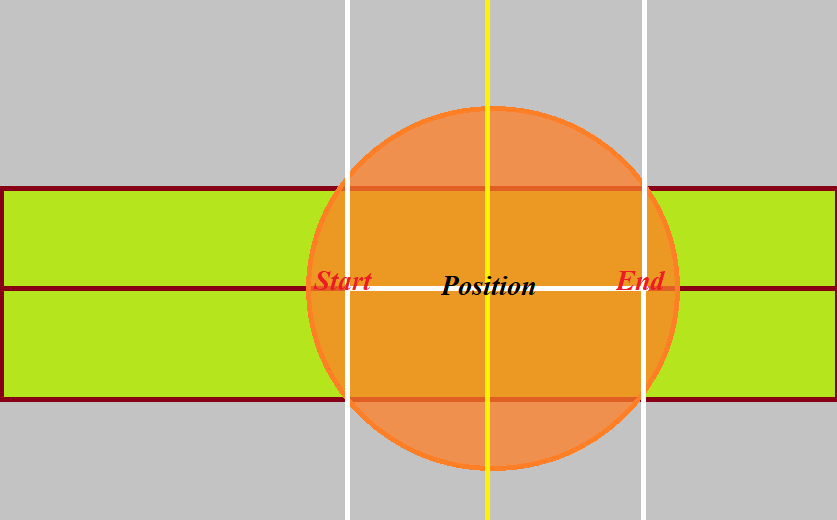
\includegraphics[width=9cm, lengh= 25cmm]{start_end.png}\\
  \caption{Reprezentare interval start - end.}
  \label{fig:start_end}
\end{figure}

Figura \ref{fig:start_end} .Exemplifică intervalul pe care udă cu exactitate aspersorul.
\end{center}
La baza principiului rezolvării acestei probleme stă Teorema lui Pitagora. Cu această teoremă se află cât acoperă cercul(adică aspersorul) curent din suprafața ierbii, sub forma unui dreptunghi. Acest lucru este realizat în funcția de tip struct intitulată \textbf{ aspenToAspenPosition}, cea menționată și în paragraful anterior. Prin \textsl{Teorema lui Pitagora} se află acea distantă față de poziția aspersorului deja știută. Astfel că variabila \textsl{halfDistanceStartEnd} care este\[radius^2 - (width/2)^2\)\] Acest lucru este exemplificat în figura de mai jos, unde \textsl{halfDistanceStartEnd} este repezentată ca „X”:
\vspace{2.5mm}
\begin{center}
\begin{figura}
  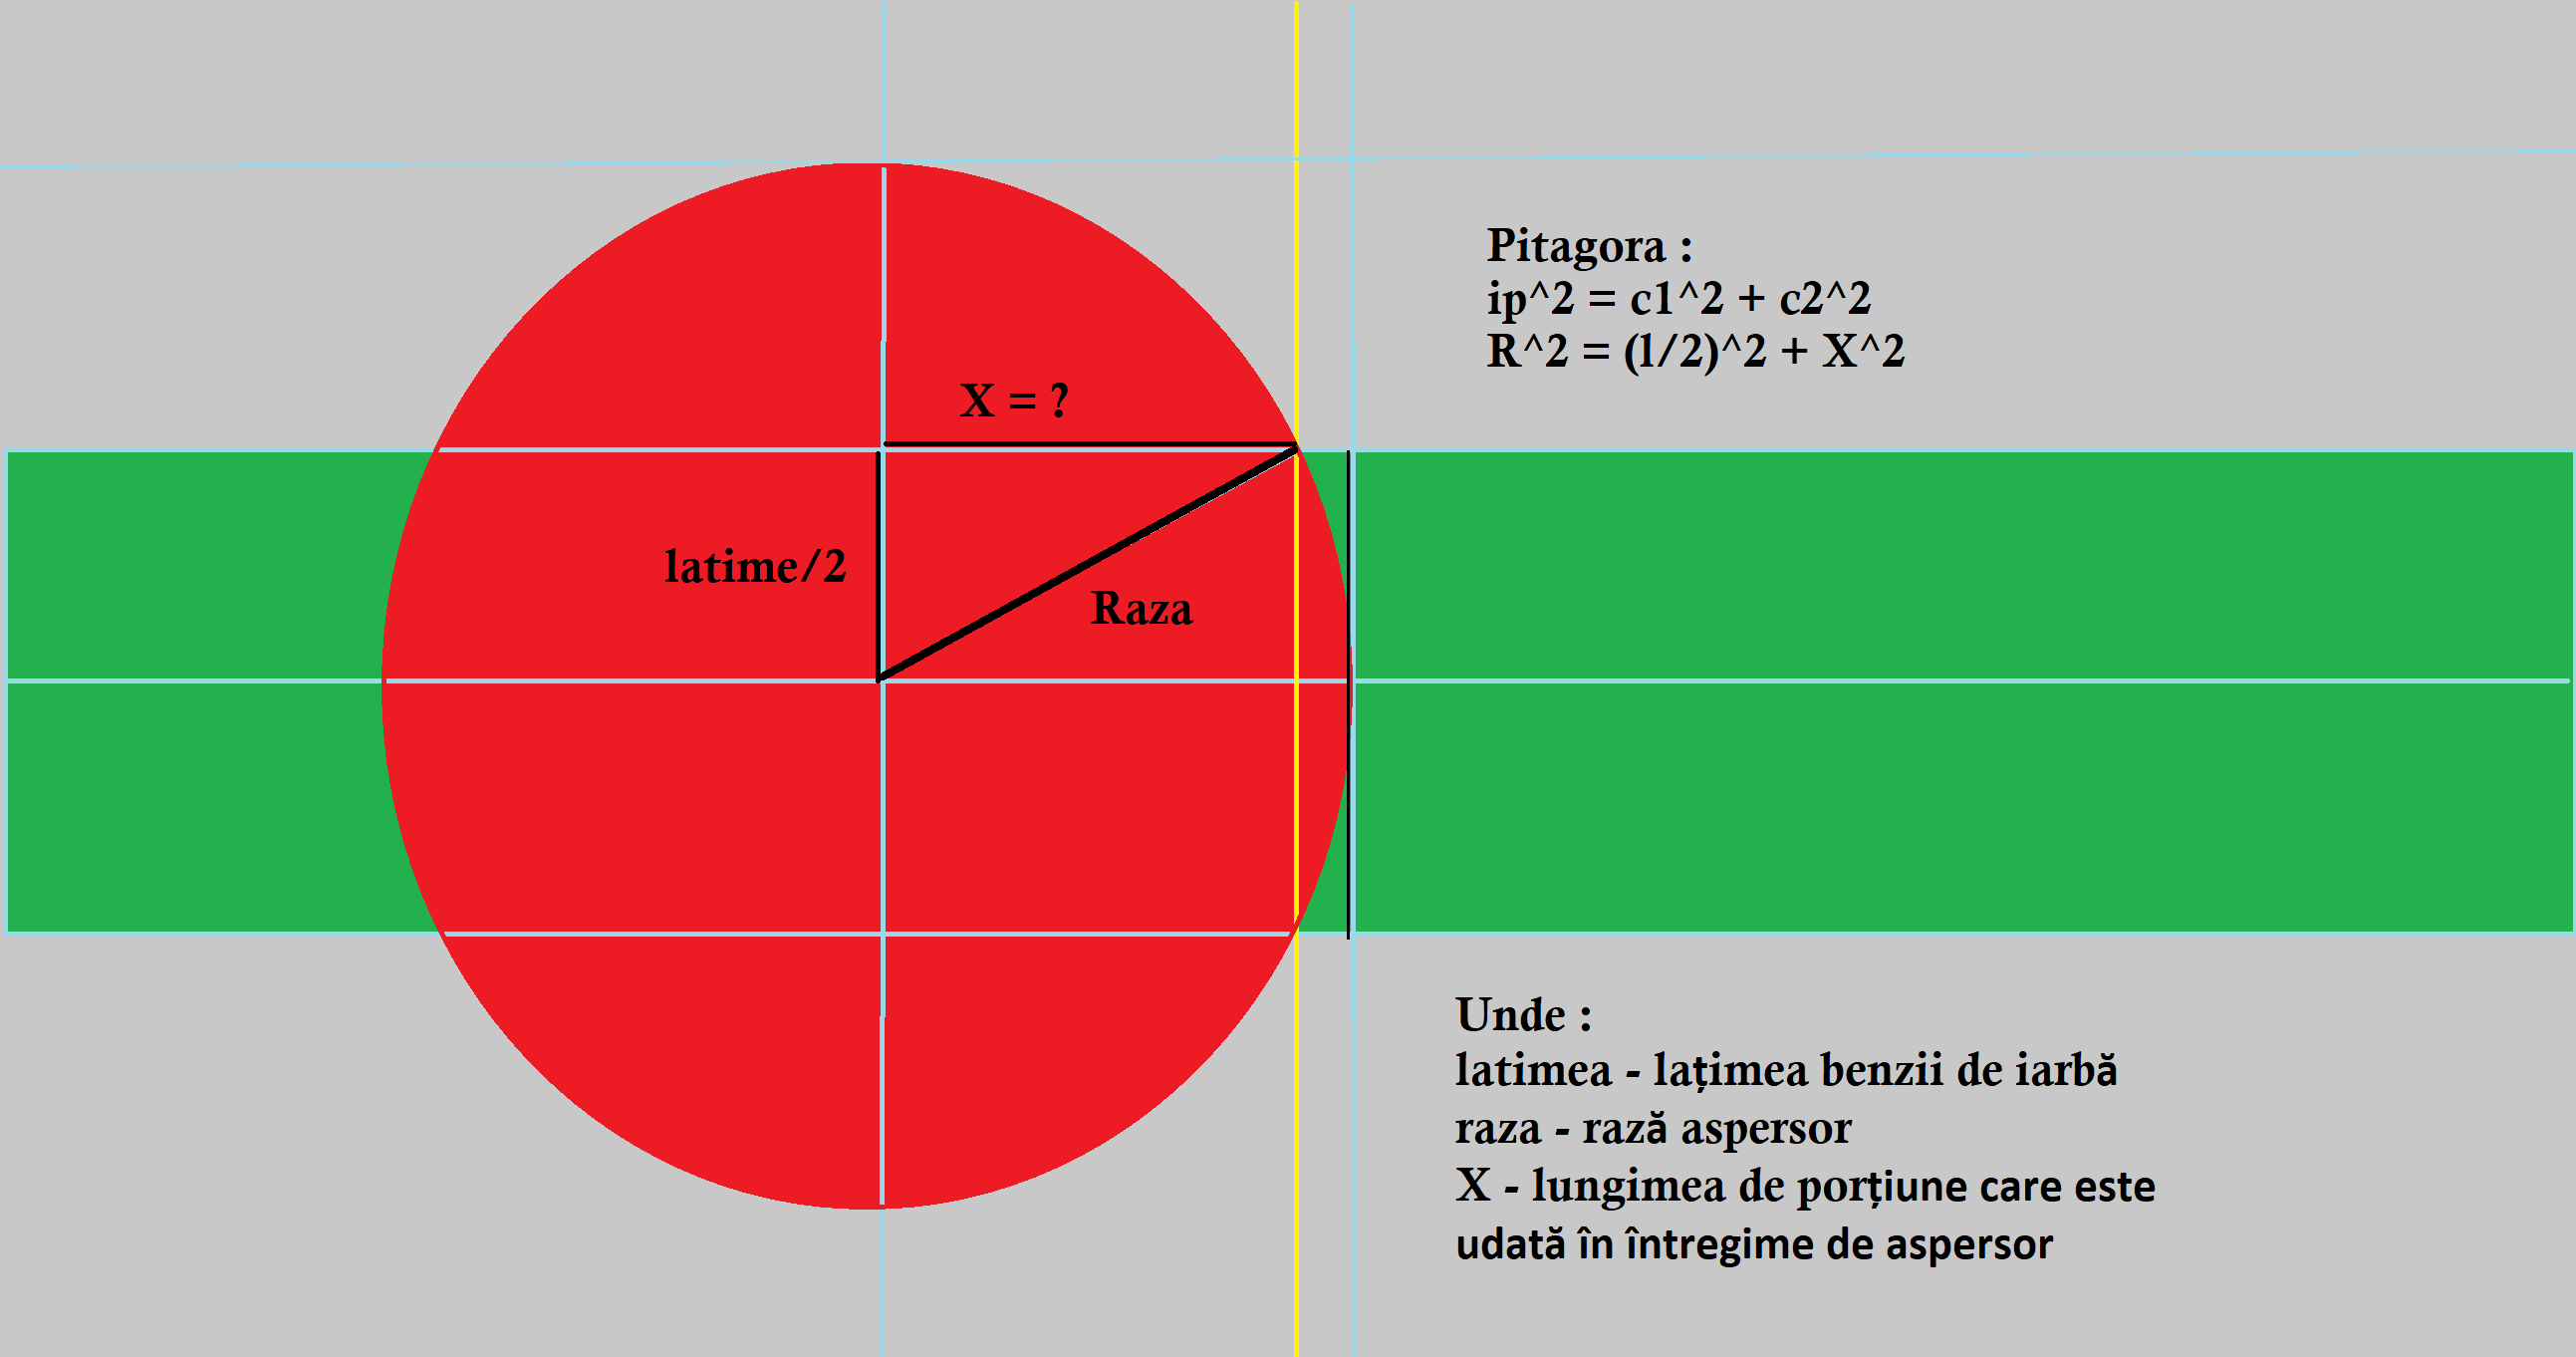
\includegraphics[width=15cm, lengh= 28cmm]{desen_pa.png}\\
  \caption{}
  \label{fig:desen_pa}
\end{figure}

Figura 2.1 .Reprezentare Teorema lui Pitagora pentru rezolvarea acestui tip de problemă.
\end{center}
\vspace{5mm}


\textbf{Fișierul \textit{modules.c}}\\
\textbf{Algoritm II \\
\textsl{Metoda II}}

\vspace{6mm}
\caption{Pseudo-codul funcției intitulată \textbf{minAspenGreedy}, cea care determină care este numărul minim de aspersoare ce trebuie pornite pentru a putea uda banda de iarbă.} \vspace{6mm}
\\
\begin{algorithm}
\begin{algorithmic}[2]
MIN-ASPEN-GREEDY( intervalAspen *coord) \\
1.\indent   \>$init minAspensors = 0$ \\
2. \indent            \> $\textbf{if} $coord_{noAspensor - 1}.final $ $ < $ $ length$ $or$ $coord_{0}.prim$ $>$ $0$ \\
3. \indent            \> \hspace{8mm} $print \hspace{1mm}"No\hspace{1mm}apensors\hspace{1mm}can\hspace{1mm}be\hspace{1mm}placed..."$ \\
4. \indent            \> \hspace{8mm}$return $ \\
5.\indent             \>  $\textbf{end if }$\\
6. \indent            \>  $minAspensors = minAspensors + 1$ \\
7.\indent             \> $\textbf{for} index1 = 1\hspace{2mm} to\hspace{2mm} noAspensors$\\
8. \indent            \>$ \hspace{8mm} \textbf{if} coord_{index1}.prim $ $ > $ $ coord_{index1 - 1}.final$ \\
9.\indent \>\hspace{16mm}$print "No aspensors can be placed...$\\
10.\indent      \>\hspace{16mm}$return$\\
11.\indent  \>\hspace{8mm}$\textbf{else} $\\
12.\indent      \> \hspace{16mm}$index2 = index1 - 1\\  
13.\indent            \>\hspace{20mm} $\textbf{while} coord_{index1}.prim <= coord_{index2}.final $  \\
14.\indent                \>\hspace{26mm} $index1 = index1 + 1$\\
15.\indent      \>\hspace{18mm} $\textbf{end while}$\\
16.\indent \>\hspace{18mm}$minAspensors = minAspensors + 1$ \\
17.\indent   \> $\textbf{end for} $\\
18.\indent \> $print "You will need a min of minAspensors" $\\
\end{algorithmic}
\end{algoritm}
\end{tabbing} 

\label{fig_alg_ex}
\end{center}
\end{figure}

\\
\\
\vspace{7mm}
\textbf{\textsl{Analiză complexitate computațională}}\\
\\
În tabelul de mai jos este exemplificat o analiză a best, worst și average case pentru algoritmii propuși, dar și o analiză pentru metoda de sortare \textbf{Bubble - sort} ce este folosită în ambele programe.

\begin{document}
\begin{center}
\begin{tabular}{ |p{2cm}||p{2.5cm}|p{2.5cm}|p{2.5cm}|  }
 \hline
 \multicolumn{4}{|c|}{Analiză Best, Worst și Average Case } \\
 \hline
 Algoritmii        & Best Case  &Worst Case &Average Case \\
 \hline
Algoritm I   
\hspace{4mm}
Metoda I    & O(1)    &O(n^2 + n) &\Theta \frac({2}{n-1})  \\
\hline
Algoritm II
Metoda II     &O(1)     &(n) & - \\
\hline
Bubble-Sort   &O(n) &O(n^2) &\Theta (n^2)\\
 \hline
 
\end{tabular}
\end{center}

\hspace{6mm}Notații asimptotice\\
{1 $<$ log n $<$ \sqrt{n} < n < nlog n < n^2 < n^3< ......< 2^n < 3^n < ..... < n^n}\\\\
Big O - $upper bound$\\
\Omega - $lower bound$\\
\Theta - $average bound$\\

Notațiile asimptotice pentru cei doi algoritmi în C :\\

\begin{document}
\begin{center}
\begin{tabular}{ |p{2cm}||p{2.5cm}|p{2.5cm}|p{2.5cm}|  }
 \hline
 \multicolumn{4}{|c|}{Notații asimpotice } \\
 \hline
 Algoritmii        &Upper bound &Lower bound &Average bound \\
 \hline
Algoritm I   
\hspace{4mm}
Metoda I    & O(n^2)-pătratic    &\Omega(nlog n) &\Theta (n^2)  \\
\hline
Algoritm II
Metoda II     &O(n)     &\Omega(n) & \Theta(n) \\
\hline

 \hline
\end{tabular}
\end{center}
\vspace{6mm}
\section{Proiectarea aplicației experimentale}

\begin{itemize}

\item
Structura de nivel \^{i}nalt a aplica\c{t}iei

\begin{figura}
  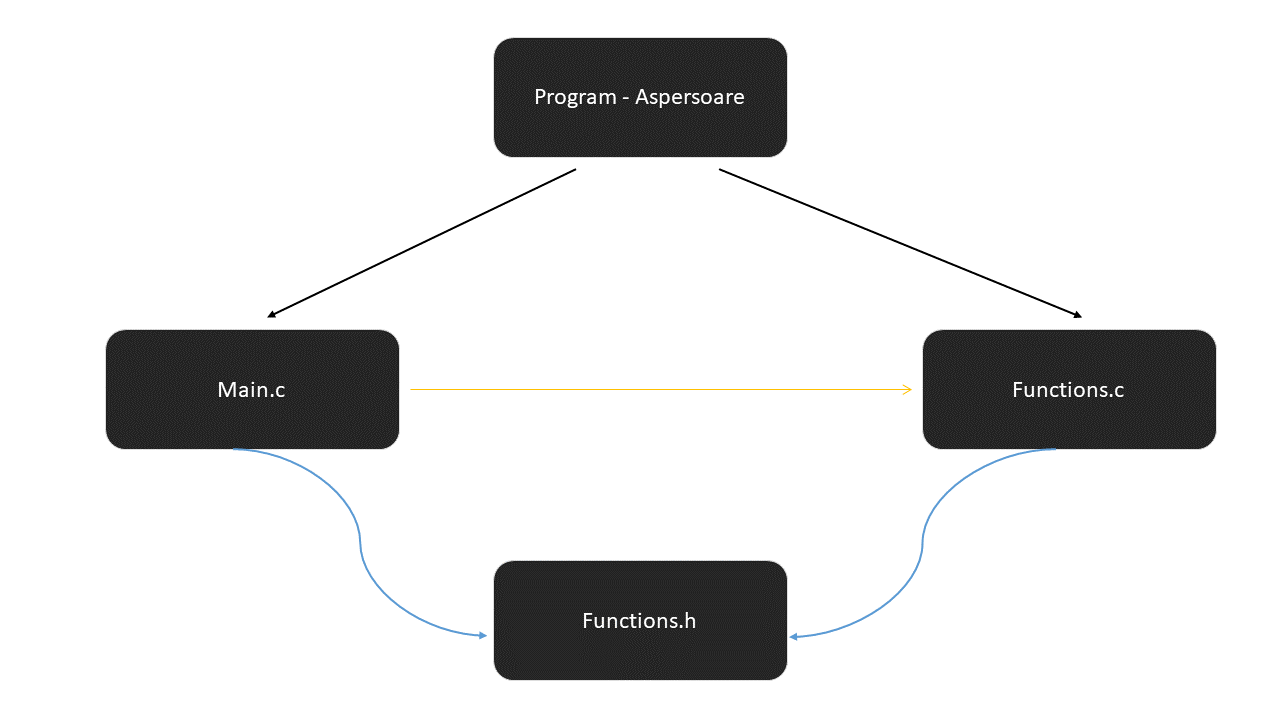
\includegraphics[width=15cm,lengh = 25cm,inner]{struct.png}\\
  \caption{}
  \label{fig:struct}
\end{figure}

Figura 3.1. Structura pentru Metoda I de program în limbaj C
\begin{center}

\begin{figura}
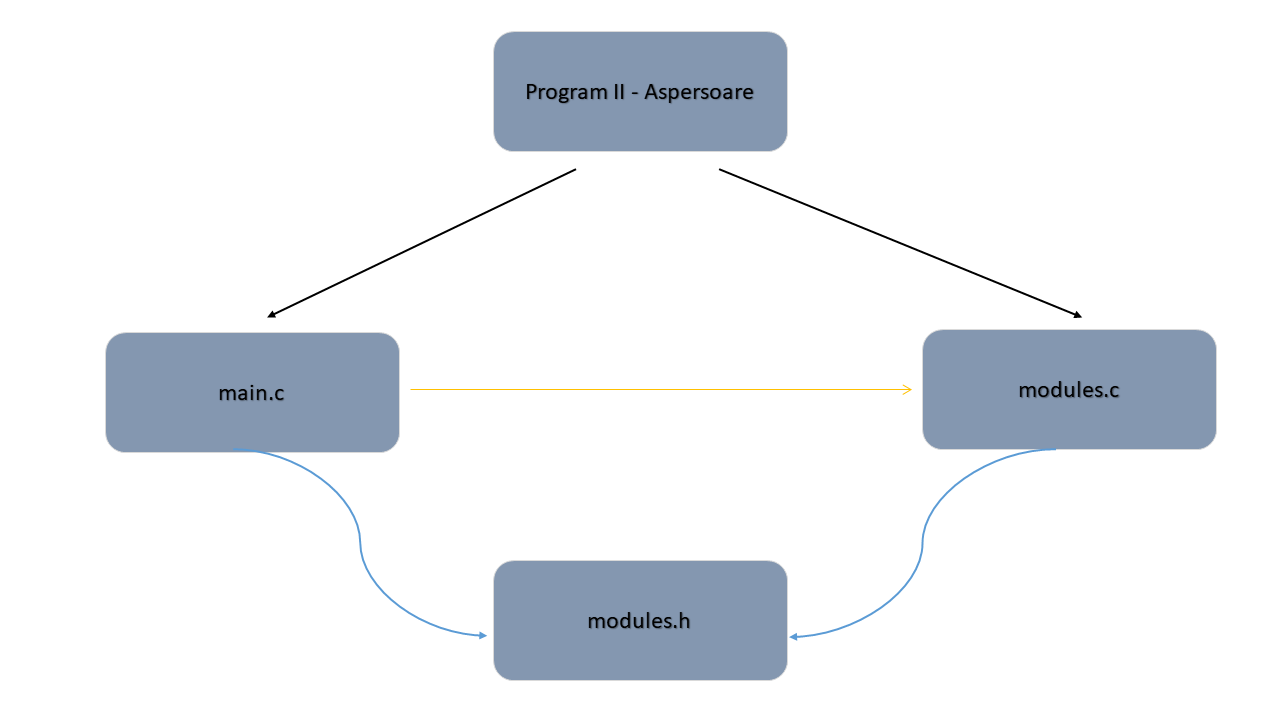
\includegraphics[width=14cm, lengh=20cm]{struct2.png}\\
  \caption{}
  \label{fig:struct2}
\end{figure}

 Figura 3.2. Structura pentru Metoda II de program în limbaj C
\end{center}
\end{itemize}
\vspace{3mm}

\begin{itemize}

\item
Descrierea mul\c{t}imii datelor de intrare
\end{itimize}\\

Datele de intrare au fost generate cu ajutorul unui generator de date. 
S-au generat date pentru lungimea, lățimea dreptunghiului, adică a benzii de iarbă, numărul de aspersoare ce sunt instalate pe banda orizontală ce străbate dreptunghiul prin mijlocul acestuia și , de asemenea, raza de operare și poziția( distanta față de capătul din stânga al liniei care străbate pe orizontal mijlocul fîșiei de iarbă).
Datele generate sunt date netriviale, acestea sunt declarate ca și \textbf{double} - pentru lățime și lungimea, rază, iar \textbf{int} pentru numărul de aspersoare și poziție.\\
Datele generate pentru intare sunt obținute aleator.
Au fost generate 10 seturi de date diferite, la fiecare set de date sunt generate numerele dintr-un anumit interval. Cum ar fi intervalul [1,1000], din aceasta au fost generate doar date ce sunt cuprinse în el, de exemplu datele din Figura 3.3., date ce se regăsesc și într-un fișier de input al programului : 

\\
\vspace{5mm}

\begin{figura}
\centering
  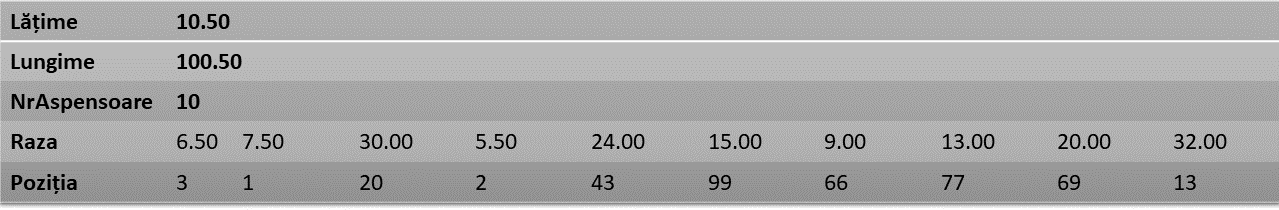
\includegraphics[width=15cm,lengh = 23cm, inner]{tabel.png}\\
  \caption{}
  \label{fig:tabel}
\end{figure}

Figura 3.3. Exemplu date de intrare generate\\
\\


Mulțimea datelor de intrare au fost generate astfel: un număr oarecare pentru lungimea benzii de iarbă, un număr oarecare pentru numărul de aspersoare, un număr oarecare pentru lățimea benzii, dar mai mic decât lungimea. Iar pentru rază și poziție, numere oarecare , în cazul poziției numere mai mici decât lungimea benzii de iarba. Raza a fost generata ca și când poate să fie mai mare decăt lățimea, nu s-au impus altfel de condiții.

\begin{itemize}
    \item Descrierea ieșirilor / rezultatelor
\end{itemize}
Primul program, adică prima metodă implementată afișează numărul minim de aspersoare necesare pentru a putea fi udată în întregime banda de iarbă.
Dar daca dorim să vedem și începutul, sfârșitul intervalului pe care udă aspersorul de-a lungul benzii(suprafața ierbii, care este sub forma unui dreptunghi, aceast interval reprezentând linia de simetrie verticală ce trabate cercul, cercul fiind o figură geometrică simetrică la fel ca și dreptunghiul), putem afișa și acest lucru. Datele vor fi afișate sub numele de \textsl{start} și \textsl{end} pentru fiecare aspersor. Un exemplu de rulaj este prezentat în figura de mai jos, acestea pot fi afișate prin apelarea funcției \textbf{printAspenArrayAndAspenPositionArray()} și înainte de a fi sortate, dar și dupa sortare: 
\\

\begin{figura}
\centering
  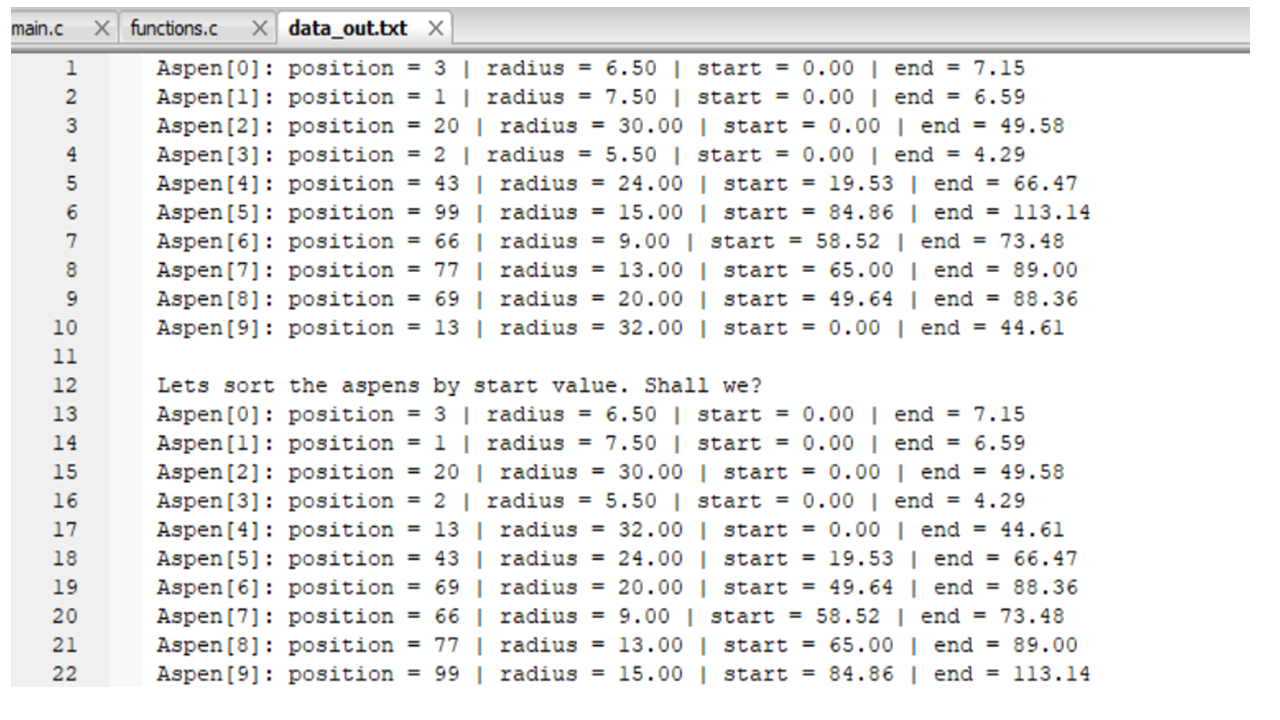
\includegraphics[width=15cm,lengh = 25cm,inner]{out.png}\\
  \caption{}
  \label{fig:out}
\end{figure}

Figura 3.4. Dacă se dorește afișarea pentru datele calculate\\

Se poate observa în Figura 3.4 că unele aspersoare au ca valoare de \textbf{start} valoarea 0. Atunci cănd punctul de \textsl{start} calculat are valoare negativă ( start$ <$ 0 ), calculat cu ajutorul variabilei \textsl{halfDistanceStartEnd} de tip double prin intermediul Teoremei lui Pitagora (de altfel partea cea mai importanta din rezolvarea problemei), această valoare este rotunjită la 0, deoarece ne dorim să fie pozitivă.\\
De asemenea, se poate afișa în fișierul de output doar numărul minim necesar de aspersoare pentru a putea fi udată fâșia de iarbă, însoțit de un mesaj corespunzător. Iar dacă banda de iarbă nu poate fi acopertiă cu datele de intrare generate, se va afișa mesaj corespunzător.\\
Cel de-al doilea program implementat, poate afișa la fel ca primul valoarea pentru începutul și sfârșitul intervalului pe care udă aspersorul.
\\O concluzie privind datele de ieșire ale celor două programe, este faptul ca la cel de-al doilea programul valoarea de început, intitulată \textbf{prim} nu mai este rotunjită la 0 ca și valoarea \textbf{start} din primul program. Astfel că, acest program calculează numărul minim de aspersoare necesare și cu valorile posibile negative ale variabile \textsl{prim}. De exemplu, în figura 3.5, se poate observa această diferență între datele de ieșire cu privire la valoriile variabilelor \textsl{prim} și \textsl{final} din cel de-al doilea program, și faptul ca acestea sunt numere fără zecimale, fiind afișate ca numere întregi, nu de tip double.



\begin{document}
\begin{center}
\begin{tabular}{ |p{2.5cm}||p{2.5cm}|  }
 \hline
 \multicolumn{2}{|c|}{Rezultate generate } \\
 \hline
 Valoare \textbf{prim}        & Valorea \textbf{final} \\
 \hline
-19.00   &45.00  \\
\hline
-10.00 & 50.00 \\
\hline
-6.50   &8.50\\
 \hline
 -3.50 & 7.50\\
 \hline
 -3.50 & 9.50\\
 \hline
 19.00 & 67.00\\
 \hline
 49.00 & 67.00\\
 \hline
 57.00 & 75.00\\
 \hline
 64.00 & 90.00\\
 \hline
 84.00 & 114.00\\
 \hline
 \hline

\end{tabular}
\end{center}
Figura 3.5 Posibile date de ieșire pentru a doua implementare
\\

Datele din Figura 3.4 și 3.5 au avut aceleași date de intrare, respectiv datele exemplificate în Figura 3.3
\begin{itemize}
    \item Lista tuturor modulelor aplicației și o scurtă descriere a lor\\
    Pentru implementare primei rezolvări:
    \begin{itemize}
        \item \textit{\textbf{main.c}} - în acest modul se citesc din multiplele fișiere datele de intrare și sunt apelate funcțiile necesare ce se află în \textsl{functions.c}, de asemenea aici se calculează timpul de execuție al algoritmului implementat.
        \item \textit{\textbf{functions.c}} - în acest modul se află funcțiile programului, ce ajută la rezolvarea problemei
        \item\textit{\textbf {functions.h}} - în acest modul sunt declarate structurile folosite pentru datele despre aspensor, cum ar fi \textbf{struct apen} și \textbf{strcut aspenPosition}, lungimea, lățimea și numărul de aspersoare, dar și prototipurile funcțiilor apelate.\\
    \end{itemize}
    Pentru implementarea celei de-a doua rezolvări:
    \begin{itemize}
         \item \textit{\textbf{main.c}} -  în acest modul se citesc din multiplele fișiere datele de intrare și sunt apelate funcțiile necesare ce se află în \textsl{modules.c}, de asemenea aici se calculează timpul de execuție al algoritmului implementat.
        \item \textit{\textbf{modules.c}} - în acest modul se află funcțiile programului, ce ajută la rezolvarea problemei
        \item \textit{\textbf {modules.h}} - în acest modul sunt declarate structurile folosite pentru datele despre aspensor, cum ar fi \textbf{struct apensor} și \textbf{strcut intervalAspen}, lungimea, lățimea și numărul de aspersoare, dar și prototipurile funcțiilor apelate.\\
    
    \end{itemize}

\end{itemize}
\begin{itemize}
    \item Lista tuturor procedurilor aplicației, grupate pe module\\
      Prima implementare: 
    \begin{itemize}
        \item main.c : 
            \begin{itemize}
                \item clock()- calculează timpul de execuție al algoritmului \textsl{ minAspensNumber()}
                \itema void arrayAspenToArrayAspenPosition () - convertește fiecare element de tipul  aspenArray in aspenPosition și le memorează in vectorul aspenPositionArray. Este o funcție de tip \textbf{void}
            \end{itemizw}
        \item functions.c: 
            \begin{itemize}
                \item void sortAspenPositionArrayByStart () - sortează crescător prin metoda Bubble - Sort aspersoarele în funcție de distanța, calculată cu Teorema lui Pitagora și scăzând poziția știută din datele problemei,față de capătul din stânga al liniei care străbate  pe orizontală mijlocul fâșiei de iarbă.Prin această sortare sunt mutate odată cu aspersorul și informațiile despre el, cum ar fi valoriile de start, end, raza, poziția.
                \item int minAspensNumber () - calculează numărul minim de aspersoare necesare prin comparare valorile de start și end. Prima dată se caută aspersoarele care au cea mai mare valoare de end și valoarea de start egală cu zero.Apoi se parcurge în continuare vectorul numir aspenPositionArray până când se ajunge la ultimul aspensor care se află la finalul benzii de iarbă și valoarea sa este mai mare sau egală cu lungimea sau nu mai avem aspersoare. Iar în final daca nu sunt suficiente aspersoare sa acopere fâșia de iarbă se va returna valoarea -1, altfel se va returna prin variabila de return \textbf{minAspens} numărul minim aflat.
                \item init(double lengthAux, double widthAux, int aspenTotalAux) - dacă se dorește și afișarea lungimii, lățimii și numărului de aspersoare.
                \item void printAspenArrayAndAspenPositionArray () - dacă se dorește să se afișeze poziția, raza, start-ul și end-ul pentru fiecare aspersor, asa cum este exemplificat în Figura3.3
            \end{itemize}
    \end{itemize}
    Cea de a doua implementare:
    \begin{itemize}
        \item main.c:
        \begin{itemize}
            \item clock() - pentru calcularea timpului de execuție a algoritmului intitulat minAspenGreedy (coord);
        \end{itemize}
        \item modules.c
        \begin{itemize}
            \item void starting(struct aspensor *properties, struct intervalAspen *coord) - determină intervalul ce are ca și capetele \textbf{prim}, \textbf{final} pentru a afla distanța pe care udă aspersorul. Parametrii semnifică tipul lui \textsl{proprieties} și \textsl{coord}, ce sunt alocați dinamic.
            \item void eliminate(struct intervalAspen *coord, double position) - elimină aspersoarele care au aceeași poziție, dar celălalt are raza mai mare, este funcție auxiliară pentru funcția ”duplicat”.Ca și parametrii avem *coord , alocat dinamic și poziția.
            \item void duplicate(struct aspensor *properties, struct intervalAspen *coord) - elimină aspersorul care se află în interiorul celuilalt aspersor, iar raza acestuia este mai mică decât cea a celuilalt. Aspersorii au aceeași poziție, dar raza diferită. 
            \item void sorting (struct intervalAspen *coord, struct aspensor *properties) - sortează crescător prin metoda Bubble - Sort aspersoarele în funcție de distanța, calculată cu Teorema lui Pitagora și scăzând poziția știută din datele problemei,față de capătul din stânga al liniei care străbate  pe orizontală mijlocul fâșiei de iarbă.Prin această sortare sunt mutate odată cu aspersorul și informațiile despre el, cum ar fi valoriile de start, end, raza, poziția.
            \item void minAspenGreedy (struct intervalAspen * coord) - calculează numărul minim de aspensoare necesare pentru a acoperi întrega bandă de iarbă folosind metoda Greedy.
        \end{itemize}
    \end{itemize}
    
\end{itemize}
\section{Date experimentale}
\begin{itemize}
    \item Descrierea algoritmului folosit pentru generarea de mulțimi de date de intrare
\end{itemize}
Algoritmul folosit pentru generarea de mulțimi de date de intrare generează valori pentru lățimea, lungimea, numărul de aspersoare și raza, poziția pentru fiecare aspersor.
Datele sunt de tipul următor:

\begin{document}
\begin{center}
\begin{tabular}{ |p{2.5cm}||p{3cm}|  }
 \hline
 \multicolumn{2}{|c|}{Tipul datelor generate } \\
 \hline
 \textbf{double}        &  \textbf{int} \\
 \hline
lungimea(length)       & numărul de aspersoare(noAspen) \\
\hline
lățimea(width) & poziția(position) \\
\hline
raza(radius) &- \\
 \hline
\hline
\end{tabular}
\end{center}

Pentru a se putea genera valori s-a folosit funcția pentru generare automată de date aleatorii \textbf{rand} .Această funcție generează un număr între o valoare maximă impusă și una minimă impusă. Valoarea de maxim poate fi modificată, deoarece a fost declarată cu macro \textbf{\#define}. 
\\ Lungimea(length) este generată între 1 și o valoare maximă defină, lățimea(width) este generată între 1 si lungimea/10, deoarece trebuie să fie o valoarea mai mică decât lungimea , iar numărul de aspersoare este o valoare intre 1 și o limită impusă, de asemenea, și aceasta definită prin \#define. Pentru raza și poziția fiecarui aspersor s-au impus astfel valorile pentru limita inferioră și cea superioară: pentru poziție valori între 0 și lungimea, iar pentru rază valorile între 0 și lungimea/8, deoarece trebuie să fie valori mai mici decât lungimea, dar si posibil mai mari decât lățimea. Toate acestea sunt afișate în fișier.\\
Datele sunt corect generate și semnificative pentru teste, deoarece pe un set mic de date au fost testate și verificate, iar acestea sunt non-triviale.
\begin{itemize}
    \item Pseudo-codul generatorului de date: 
\end{itemize}
\begin{algorithm}
\begin{algorithmic}
Funcția pentru a genera date aflate între anumite limite(limită superioară și inferioară)\\
RANDOM-NUMBER(min, max) \\
1.\indent   \> $return (rand()* (max - min)) / RAND-MAX + min$  \\
\\
În\hspace{2mm} main : \\
1.\indent $Se declară un fișier pentru output$\\
2. \indent            \>$length = RANDOM-NUMBER(1, maxim)$ \\
3. \indent            \>\hspace{4mm} $print length$\\
4. \indent            \> $width = RANDOM-NUMBER(1 , length/10) $ \\
5.\indent             \> \hspace{4mm} $print width$\\
6. \indent            \>  $noAspen = RANDOM-GENERATOR(1, limit)$ \\
7.\indent             \> \hspace{4mm}$print noAspen$ \\
8.\indent \>$ \textbf{for} iter  0 \textbf{to} noAspen$\\
10.\indent      \>\hspace{4mm}$ print RANDOM-NUMBER(0, length)$\\
11.\indent       \>\hspace{4mm}$print RANDOM-NUMBER(0, length/8)$ $\\
\begin{itemize}
    \item  Am implementat acest cod din C și în Python pentru a putea observa diferețele dintre cele două limbaje. Pentru ambele implementări am ales aceleași limite inferioare și superioare. În plus, față de implementările pentru rezolvare în C, în programul din Python am adaugat  și generatorul de date. Astfel că generatorul generează date într-un fișier, iar de acolo sunt luate în mod direct de către programul principal ca mulțimi de date de intrare. S-au generat și în Python, la fel ca pentru programele în C, 10 seturi de date de intrare. Am adăugat acest generator doar pentru unul dintre programele în Python, este atașat în programul care nu conține class, am încercat să modific unul dintre programele din C ce conțin amândouă  \textbf{struct}, în Python într-un program care nu se folosește de \textbf{class}, dar care urmărește același principiu de rezolvare a problemei.
    
    \end{itemize}

\end{algorithmic}
\end{algoritm}
\end{tabbing} 

\label{fig_alg_ex}
\end{center}
\end{figure}
\section{Rezultate și concluzii}
\begin{itemize}
    \item Descrierea datelor de ieșire obținute folosind implementările în C și Python (comparație)
    \begin{itemize}
    \item Pentru implementările în C datele de ieșire sunt afișate în fișiere, câte un fișier separat pentru fiecare mulțime de date de intrare, iar datele de ieșire procesate de implementările în Python sunt afișate la ecran pentru unul dintre programe(program I), pentru celălalt intitulat Program II afișarea se face în fișier, dar  citirea mulțimilor se face din fișier în ambele implementări. În ambele implementări, atât Python cât și C, este specificat atunci când o mulțime de date nu cuprinde date necesare pentru a putea uda banda de iarbă, acest lucru este marcat cu câte un mesaj corespunzător, precum : „There aren't enough aspensors to cover the entire length/rectangle” sau în implementarea în Python: „None”.
    \item O altă precizare importantă mai este faptul că ambele coduri în C au aceleași mulțimi de date de intrare, iar primul program în Python (Program I), cel care conține integrat în program un generator de date, a conținut datele ce se regăsesc în fișierele de intrare doar o singură dată, altfel că o singură dată au fost putute compara toate implementările. De asemenea, pentru acele date de intrare s-a putut observa faptul că rezultatele sunt ușor diferite, deoarece în cazul codurilor în C, Algoritmul I este diferit de Algoritm II, astfel că exită o marjă de eroare de un aspensor între cele două implementări în C (acest lucru depinde de tipul datelor, adică din ce interval fac parte). Deoarece primul cod rotunjește la valoarea zero , poziția de start a unui aspensor atunci când aceeasta prin calculul efectuat cu Teorema lui Pitagora dă o valoare negativă, iar în cel de-al doilea, aflarea numărului minim de aspersoare se face indiferent daca acea valoare, numită îîn acest algoritm prim este negativă sau nu. 
    \item Din păcate, al doilea cod în Python nu îmi afișează numărul minim de aspersoare, aceasta calculează doar valorile lui \textsl{prim} și \textsl{final}, pe care le afișează în fișier.
\end{itemize}
    \item Timpul de execuție al algoritmilor pentru fiecare mulțime de date(acest timp a fost calculat cu ajutorul funcției clock). 
    \item Intervalul pentru fiecare algoritm corespunzător unei anumite mulțimi de date variază între valorile cuprinse în acel interval, după cel puțin 3 teste ale algortimului.
  \end{itemize}
În tabelul de mai jos este exemplificat timpul de execuție pentru fiecare algoritm implementat pe o anumită mulțime de date.
  
  
\begin{document}
\begin{center}
\begin{tabular}{ |p{3cm}||p{3cm}|p{3cm}|  }
 \hline
 \multicolumn{3}{|c|}{Timp de execuție } \\
 \hline
 \textbf{Algoritm I}        &  \textbf{Algoritm II}& \textbf{Interval mulțime date} \\
 \hline
[0.117s, 0.138s]       & [0.119s, 0.126s]& [1,200] \\
\hline
\hline
[0.167s, 0.208s]       & [0.120s, 0.145s]& [1,50] \\
\hline\hline
[0.151s, 0.178s]       & [0.141s, 0.191s]& [1,10] \\
 \hline\hline
 [0.102s, 0.151s]       & [0.105s, 0.147s]& [10,600] \\
\hline\hline
[0.111s, 0.196s]       & [0.104s, 0.127s]& [50,300] \\
\hline\hline
[0.138s, 0.177s]       & [0.096s, 0.106s]& [1,1000] \\
\hline\hline
[0.125s, 0.177s]       & [0.100s, 0.136s]& [1,100] \\
\hline\hline
[0.107s, 0.115s]       & [0.113s, 0.139s]& [100,10000] \\
\hline\hline
[0.107s, 0.124s]       & [0.106s, 0.163s]& [1,5000] \\
\hline\hline
[0.101s, 0.157s]       & [0.095s, 0.158s]& [1000,100000] \\
\hline
\hline
\end{tabular}
\end{center}
\begin{itemize}
    \item Astfel din tabelul prezentat se observă media timpilor de execuție reprezentat și prin diagrama de mai jos.
    \item Se poate observa cum variază timpul fiecarui algoritm în funcție de mulțimea datelor de intrare.
\end{itemize}

\vspace{5mm}
\begin{figura}
\centering
  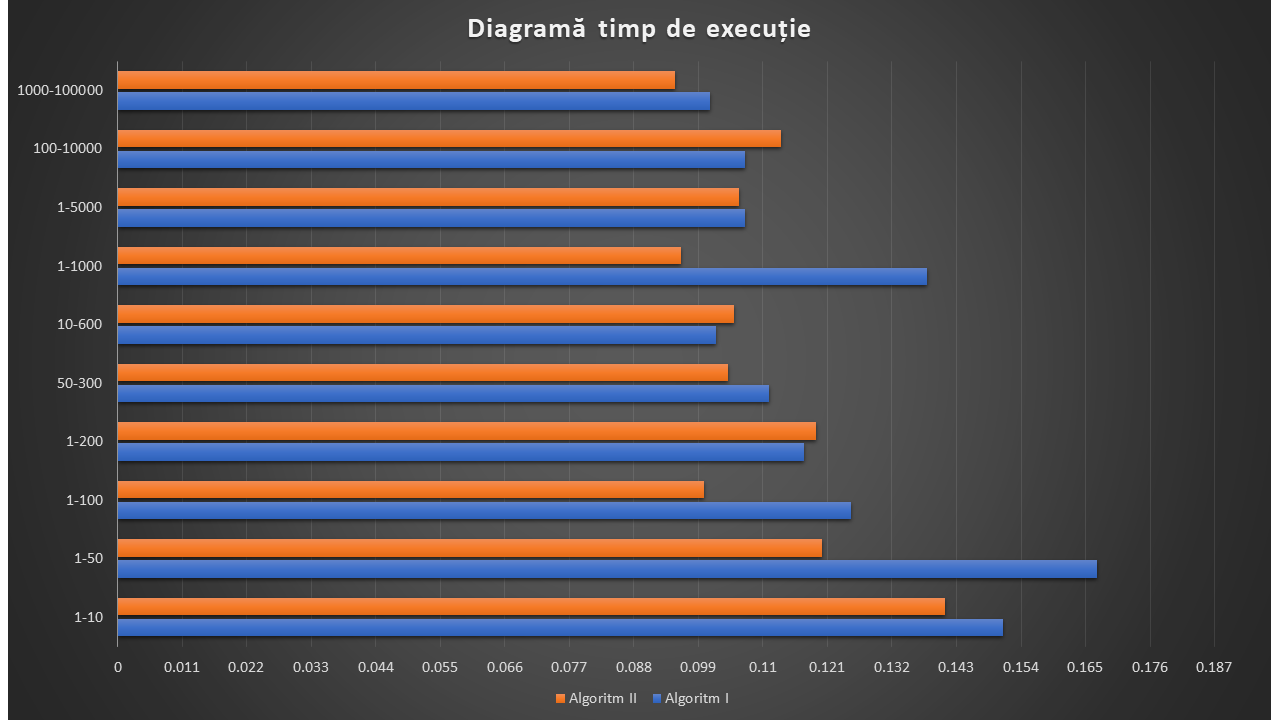
\includegraphics[width=15cm,lengh = 25cm,inner]{grafic.png}\\
  \caption{}
  \label{fig:grafic}
\end{figure}
Figura 5.1 Diagramă pentru variația timpului de execuție\\
\vspace{10mm}
\end{itemize}
\begin{itemize}

\itemÎn urma analizei acestei diagrame se poate observa că Algoritmul I are un timp de execuție mai mare decât Algoritmul II, ceea ce era de aștept, deoarece Algoritmul I are o complexitate de O{ (\(n^2\))}, iar cel de-al doilea complexitatea O(n), astfel se efectuează mai multe operații, necesitând timp mai mult.
\end{itemize}
\vspace{5mm}
\begin{figura}
\centering
  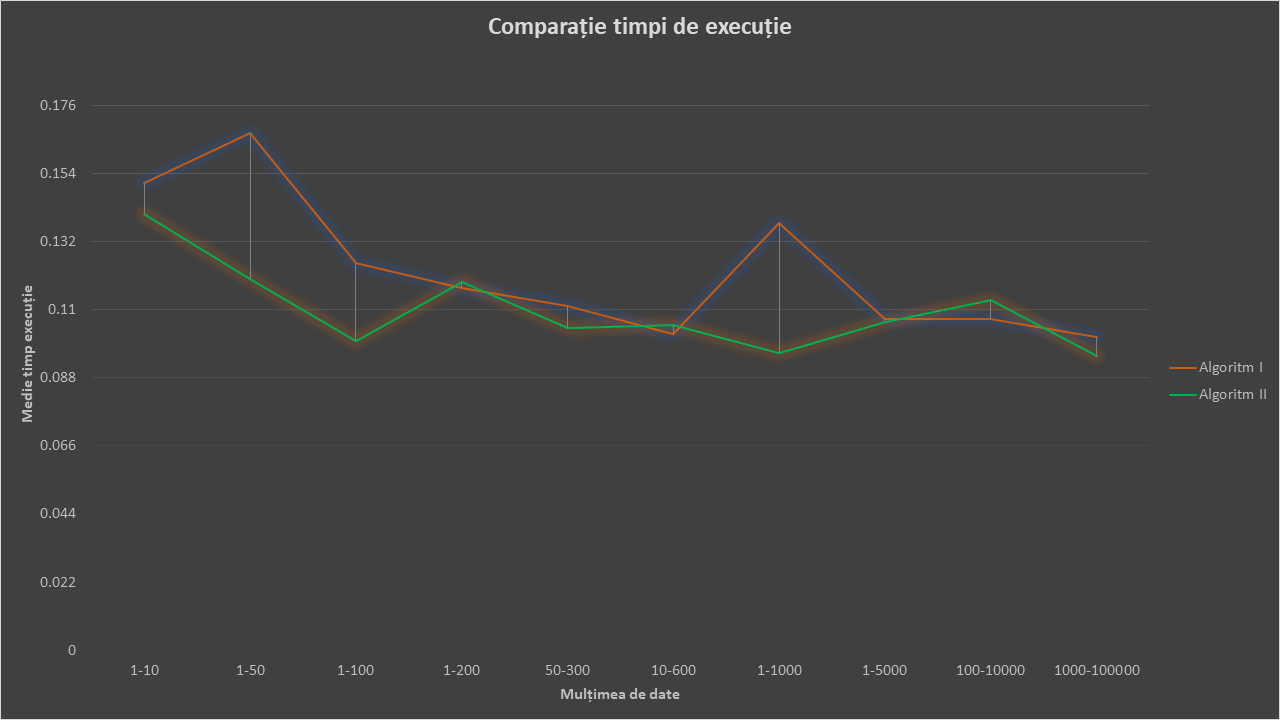
\includegraphics[width=15cm,lengh = 25cm,inner]{grf2.png}\\
  \caption{}
  \label{fig:grf2}
\end{figure}
Figura 5.1 Diagramă comparație timp de execuție\\

\begin{itemize}
    \item Timpul de execuție pentru codurile în Python nu au putut fi calculate, deoarece folosind funcția time() din Python, aceasta îmi afișează mereu valaorea zero, deși este testată pe date de intrare diferite. 
\end{itemize}

\begin{itemize}
    \item Concluzii :
    \begin{itemize}
        \item Cea mai mare provocare și intersantă parte cu privire la această temă a fost să gasesc o complexitate cât mai mică, preferabil liniară, cât mai optimă și de asemenea implementarea a doi algoritmi diferiți pentru aceeași problemă, dar și faptul să folosesc date de intrare netriviale. Datele fiind foarte importante în testarea algoritmilor.
        \item Iar ca direcție viitoare privind extinderea studiului, ar fi aceea de a schimba primul algoritm scris în C, într-unul cu o complexitate mai mica, o idee ar fi implementarea cu arbori și să reuseșesc să fac complexitatea O(nlogn).
        \item Tot pentru primul algoritm în C, Algoritm I, se poate optimiza dacă aș stoca un aspersor ca o singură strcutură care să aibă : position, radius, start, end.
    \end{itemize}
\end{itemize}

% bibliography
\section{Referințe bibliografice}

	\bibitem{cormen09}
	  [1] Thomas H. Cormen and Charles E. Leiserson and Ronald L. Rivest and Clifford Stein,
	  \emph{Introduction to Algorithms}.
	  MIT Press,
	  3rd Edition,
	  2009, accesat în aprilie 2020

    \bibitem{latex}
     [2] \LaTeX~project site,
     \url{https://www.overleaf.com/learn/how-to/Creating_a_document_in_Overleaf},
     accesat în aprilie 2020.

     \bibitem{cormen-latex}
     [3] Python 
      \url{https://www.w3schools.com/python/default.asp} , accesat în mai 2020
      \bibitem{latex}
      [4] Metoda Greedy
      \url{https://www.geeksforgeeks.org/greedy-algorithms/}, accesat aprilie 2020
       \bibitem{latex}
     [5] Random generator
      \url{https://www.tutorialspoint.com/c_standard_library/c_function_rand.htm}, accesat aprilie 2020
      

\end{thebibliography}
\end{document}



